% !TeX spellcheck = es_ES
\documentclass[titlepage]{article}
\usepackage[utf8]{inputenc}
\usepackage[letterpaper, margin=2.5cm]{geometry}
\usepackage[spanish]{babel}
\usepackage{listings}
\usepackage{url}
\usepackage{float}
\usepackage{graphicx} 
\usepackage{color}

\usepackage[nottoc,notlot,notlof]{tocbibind}
\definecolor{dkgreen}{rgb}{0,0.6,0}
\definecolor{gray}{rgb}{0.5,0.5,0.5}
\definecolor{mauve}{RGB}{253,151,31}
\definecolor{deepred}{RGB}{249,38,114}

\lstset{frame=tb,
  language=Python,
  aboveskip=3mm,
  belowskip=3mm,
  showstringspaces=false,
  columns=flexible,
  numbers=left,
  stepnumber=1,
  basicstyle={\small\ttfamily},
  numberstyle=\tiny\color{gray},
  keywordstyle=\color{blue},
  commentstyle=\color{dkgreen},
  stringstyle=\color{mauve},
  breaklines=true,
  breakatwhitespace=true,
  tabsize=2,
  morekeywords={self, append},
  emph={Transicion, __init__, True, False, __str__, AFN, AFD, Analizador},
  emphstyle=\color{deepred}
}

\title{Reporte: Práctica 2}
\author{Barrera Pérez Carlos Tonatihu \\ Profesor: Saucedo Delgado Rafael Norman \\ Compiladores \\ Grupo: 3CM6 }
\begin{document}
  \maketitle
  \tableofcontents
  \newpage
  \section{Introducción}
  Existen diferentes formas para poder construir un autómata finito no determinista a partir de una expresión regular, en esta práctica 
  se utilizo la construcción de Thomson \cite{compis} con este algoritmo cada vez que se representa algún símbolo, una unión, concatenación, 
  cerradura de Kleene o positiva se crean dos nuevos estados. El algoritmo consiste en lo siguiente:
  \begin{itemize}
   \item Para $ \epsilon $ se construyen dos estados y la transición entre ellos se etiqueta con épsilon como en la figura \ref{fig:e}
      \begin{figure}[H]
	\begin{center}
	  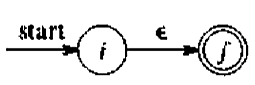
\includegraphics[width=4cm]{e.png}
	  \caption{Épsilon representado en un autómata}
	  \label{fig:e}
	\end{center}
      \end{figure}
    \item Para algún símbolo del alfabeto se realiza lo mismo que para $ \epsilon $ pero esta vez se etiqueta con el respectivo símbolo como el ejemplo 
    de la figura \ref{fig:a}.
      \begin{figure}[H]
	\begin{center}
	  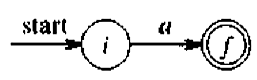
\includegraphics[width=4cm]{a.png}
	  \caption{Representación de la transición de un estado a otro a través del símbolo $a$.}
	  \label{fig:a}
	\end{center}
      \end{figure}
    \item La unión de dos expresiones regulares $ s $ y $ t $ se representa a través del uso de transiciones épsilon como se muestra en la figura 
    \ref{fig:union}.
      \begin{figure}[H]
	\begin{center}
	  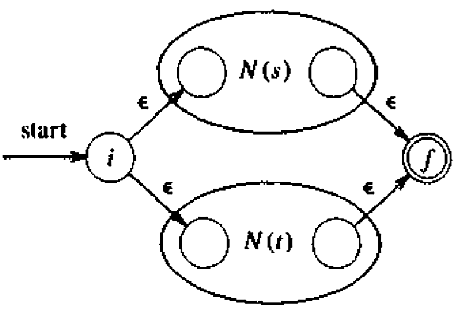
\includegraphics[width=6cm]{union.png}
	  \caption{Unión de dos expresiones regulares ($s|t$) representadas en un AFN-$\epsilon$.}
	  \label{fig:union}
	\end{center}
      \end{figure}
    \item La concatenación de dos expresiones regulares $ s $ y $ t $ se realiza tomando el estado inicial de la transición $ t $ y convirtiéndolo 
    en el estado final de la transición producida por la expresión regular $ s $ como en la figura \ref{fig:concatenacion}.
      \begin{figure}[H]
	\begin{center}
	  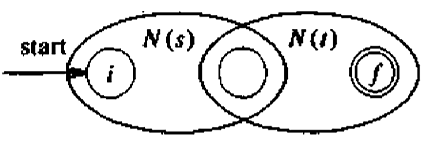
\includegraphics[width=6cm]{concatenacion.png}
	  \caption{Concatenación ($st$) mediante la fusión de un estado final y uno inicial respectivamente.}
	  \label{fig:concatenacion}
	\end{center}
      \end{figure}
    \item La cerradura de Kleene de una expresión regular $ s^* $ se realiza usando transiciones épsilon entre los estados que componen esta expresión 
    Esto se muestra en la figura \ref{fig:cerradura}.
      \begin{figure}[H]
	\begin{center}
	  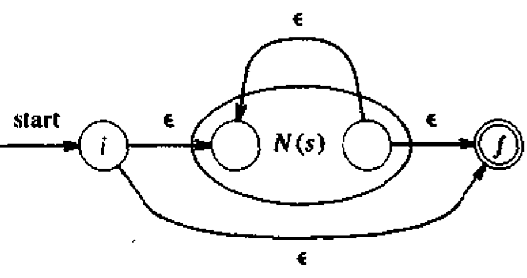
\includegraphics[width=8cm]{cerradura.png}
	  \caption{Cerradura ($s^*$).}
	  \label{fig:cerradura}
	\end{center}
      \end{figure}
    \item La cerradura positiva es similar a la de Kleene pero esta no realiza una transición del estado inicial al final.
  \end{itemize}
  Finalmente, para la evaluación de la expresión regular primero la pasamos a postfijo con el algoritmo shunting yard \cite{postfijo} que se utiliza para la 
  evaluación de expresiones matemáticas pero adaptándolo a expresiones regulares.
  \section{Desarrollo}
  La siguiente clase contiene todos los métodos necesarios para obtener un AFN a través de una expresión regular los métodos mas importantes de esta clase son:
  
  \begin{itemize}
  	\item \emph{convertir\_postfijo}. Este método genera la expresión en postfijo mediante el uso del algoritmo shuting yard \cite{postfijo} por lo que utilizamos una pila y una cola, en la pila se almacenan los paréntesis y operadores que irán saliendo de esta pila y se pondrán en la cola dependiendo de la lectura de carácter que se haga. 
  	Por otro lado, en la cola se guardara la salida en postfijo que después sera utilizada por el método generar autómata
  	\item \emph{generar\_automata}. Este método toma la salida del método anterior y haciendo uso de las construcciones de Thomson obtiene el autómata Para hacer esto utiliza una pila donde iremos guardando las transiciones que se generen y después sacándolas cuando sea necesario volver a utilizarlas y formar una nueva transición, del mismo modo guardara las transiciones resultantes, el alfabeto y los estados inicial y final en una instancia de la clase \emph{AFN} para después ser usada en la evaluación de cadenas.
  \end{itemize} 
  \begin{lstlisting}
from automata.automatas import Transicion
from automata.automatas import AFN

class Analizador:
	def __init__(self):
		self.salida_postfijo = list()
		self.transiciones = list()
		self.pila_transiciones = []
		self.POSITIVA = 0
		self.KLEENE = 1
		self.AFN = AFN()
	
	def mostar_expresion_postfijo(self):
		print(self.salida_postfijo)
	
	def mostar_automata(self):
		print('Inicial: %s Finales: %s' % (self.AFN.estado_inicial, self.AFN.estados_finales))
		print("Transiciones:")
		for t in self.AFN.transiciones:
		print(t)
	
	def convertir_postfijo(self, cadena):
		pila = []
		punto = False
		for c in cadena:
			if c == '(':
				if punto:
					while len(pila) > 0 and (pila[-1] == '+' or pila[-1] == '*'):
						self.salida_postfijo.append(pila.pop())
					pila.append('.')
					punto = False
				pila.append(c)
			elif c == ')':
				punto = True
				while len(pila) > 0 and pila[-1] != '(':
					self.salida_postfijo.append(pila.pop())
				try:
					pila.pop()
				except IndexError as e:
					raise e
			elif c == '+' or c == '*':
				self.salida_postfijo.append(c)
			elif c == '|':
				while len(pila) > 0 and (pila[-1] == '+' or pila[-1] == '*' or pila[-1] == '.'):
					self.salida_postfijo.append(pila.pop())
				pila.append(c)
				punto = False
			else:
				if punto:
					while len(pila) > 0 and (pila[-1] == '+' or pila[-1] == '*'):
						self.salida_postfijo.append(pila.pop())
				pila.append('.')
				punto = True
				self.salida_postfijo.append(c)
		
		while len(pila) > 0:
			self.salida_postfijo.append(pila.pop())
	
	def generar_automata(self):
		inicial = 1
		final = 2
		self.AFN.alfabeto.add('e')
		for c in self.salida_postfijo:
			if c == '*':
				print('CERRADURA KLEENE')
				s = self.pila_transiciones.pop()
				self.cerradura(s, self.KLEENE)
			elif c == '+':
				print('CERRADURA DE POSITIVA')
				s = self.pila_transiciones.pop()
				self.cerradura(s, self.POSITIVA)
			elif c == '|':
				print("UNION")
				s = self.pila_transiciones.pop()
				t = self.pila_transiciones.pop()
				i1 = Transicion(s[1] + 1, s[0], 'e')
				i2 = Transicion(s[1] + 1, t[0], 'e')
				f1 = Transicion(s[1], s[1] + 2, 'e')
				f2 = Transicion(t[1], s[1] + 2, 'e')
				self.pila_transiciones.append([s[1] + 1, s[1] + 2])
				self.transiciones.extend((i1, i2, f1, f2))
			elif c == '.':
				print('CONCATENACION')
				t = self.pila_transiciones.pop()
				s = self.pila_transiciones.pop()
				for aux in self.transiciones:
					if aux.siguiente == s[1]:
						aux.siguiente = t[0]
				self.pila_transiciones.append([s[0], t[1]])
			else:
				print('ESTADO')
				if self.pila_transiciones.__len__() > 0:
					inicial = self.pila_transiciones[-1][1] + 1
					final = inicial + 1
				transicion = Transicion(inicial, final, c)
				self.pila_transiciones.append([inicial, final])
				self.transiciones.append(transicion)
				self.AFN.alfabeto.add(c)
		
		self.AFN.agregar_inicial(self.pila_transiciones[0][0])
		self.AFN.agregar_finales({self.pila_transiciones[0][1]})
		self.AFN.transiciones = self.transiciones
	
	def cerradura(self, s, tipo):
		i1 = Transicion(s[1] + 1, s[0], 'e')
		s1 = Transicion(s[1], s[0], 'e')
		s2 = Transicion(s[1], s[1] + 2, 'e')
		self.pila_transiciones.append([s[1] + 1, s[1] + 2])
		self.transiciones.extend((i1, s1, s2))
	
		if tipo == self.KLEENE:
			i2 = Transicion(s[1] + 1, s[1] + 2, 'e')
			self.transiciones.append(i2)
  \end{lstlisting}
  
  El resto de métodos solo son auxiliares y sirven para mostrar el estado del autómata o para imprimir la cadena en postfijo. 
  
  \section{Resultados}
  A continuación se presenta el resultado de la implementación de la clase \emph{Analizador} en donde se convierte una expresión regular 
  a un AFN para después evaluar algunas cadenas y ver si son validas. Las pruebas se realizaron con el siguiente código, el cual ocupa la clase 
  \emph{AFN} que se construye gracias a la clase \emph{Analizador} para poder llevar a cabo la evaluación de algunas cadenas.
  
  \begin{lstlisting}
  def correr_analizador():
	  print("Generando el automata de la expresion: (a|b)*abb ...")
	  analizador = Analizador()
	  # Transformamos la expresion a postfijo
	  analizador.convertir_postfijo('(a|b)*abb')
	  analizador.mostar_expresion_postfijo()
	  # Creamos el AFN a partir de la expresion en postfijo
	  analizador.generar_automata()
	  analizador.mostar_automata()
	  # Probamos nuestro automata con algunas cadenas
	  print("Pruebas sobre el automata generado...")
	  automataAFN = analizador.AFN
	  for n in range(5):
		  cadena = input("-Ingresa una cadena: ")
		  print("La cadena es:")
		  if automataAFN.evaluar_cadena(cadena):
		  	print("Valida")
		  else:
		  	print("No valida")
  \end{lstlisting}
  
  \begin{figure}[H]
    \begin{center}
      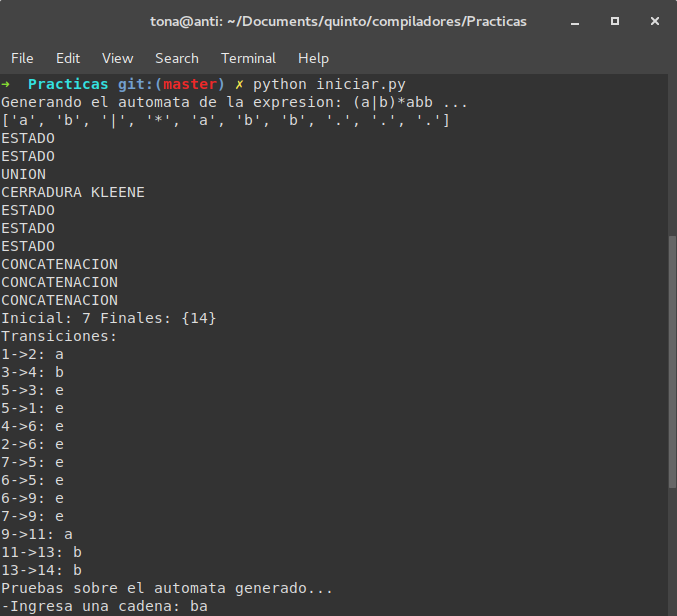
\includegraphics[width=14cm]{generacion.png}
	\caption{Transformando la expresión regular $ (a|b)^{*}abb $ a su respectivo autómata}
	\label{fig:generacion}
    \end{center}
  \end{figure}
  
  Como se puede observar en la figura \ref{fig:generacion} la expresión regular se pasa a notación posfija y después se puede observar como se realiza 
  la creación de las transiciones, lo siguiente que aparece es mostrar los estados inicial y final y finalmente se muestran las transiciones resultantes. 
  
  Después se realizaron pruebas sobre el autómata que se genero de forma similar a la práctica anterior.
  
  \begin{figure}[H]
    \begin{center}
      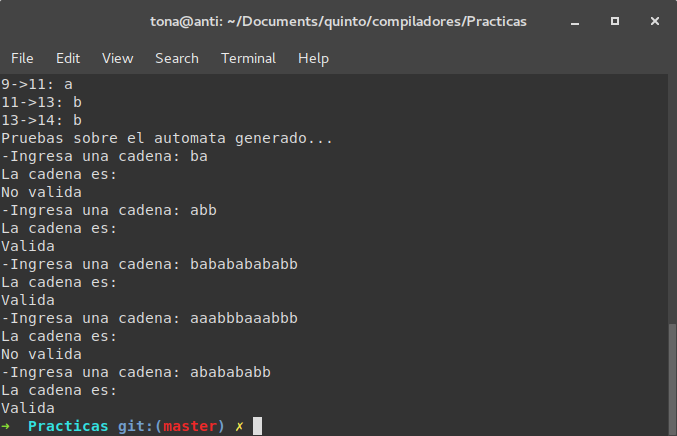
\includegraphics[width=14cm]{pruebas.png}
	\caption{Pruebas sobre el autómata generado.}
	\label{fig:pruebas}
    \end{center}
  \end{figure}
  
  La generación del autómata se realizo de forma correcta (figura \ref{fig:pruebas}), ya que la evaluación de las cadenas fue satisfactoria esto quiere decir que las transiciones 
  que se muestran en la figura \ref{fig:generacion} no tuvieron errores.
  
  \section{Conclusiones}
  La elaboración de esta práctica fue un poco más sencilla que la anterior debido a que solo consistió en implementar el algoritmo de Thomson 
  y con ello poder construir cualquier AFN, la parte complicada de modelar este algoritmo fue la concatenación ya que requirió unos pasos extra 
  a diferencia del resto de construcciones. 
  
  Y como se pudo observar en las pruebas la conversión de expresión regular a autómata se realiza correctamente. 
  Esto demuestra la versatilidad que tienen las expresiones regulares y los autómatas además de que sera de 
  mucha utilidad cuando realicemos nuestro analizador léxico que su principal tarea es revisar el vocabulario de nuestro compilador.
  \bibliography{bibliografia} 
  \bibliographystyle{ieeetr}
\end{document}
